\documentclass[11pt,a4paper]{article}

\usepackage[margin=1in]{geometry}
\usepackage{amsmath,amssymb}
\usepackage{graphicx}
\usepackage{booktabs}
\usepackage{hyperref}
\usepackage{xcolor}
\usepackage{caption}
\usepackage{subcaption}
\usepackage{enumitem}
\usepackage{parskip}
\usepackage{microtype}
\usepackage{float}

\hypersetup{colorlinks=true, linkcolor=blue, citecolor=blue, urlcolor=blue}

\title{\textbf{AE646 - Interim Report (Stage 2)}\\[0.5em]
\large \textbf{Operator Learning for Parametric Darcy Flow: FNO vs\ MLP Baseline}}
\author{\textbf{Team - PINNacles}}
\date{\textbf{18th September 2026}}

\begin{document}
\maketitle

% ─────────────────────────────────────────────────────────────────────────────
\section{Introduction}

Traditional numerical solvers such as Finite Difference Methods (FDM) and Finite Element Methods (FEM) require re-solving the full PDE for every new set of parameters, imposing prohibitive computational cost when thousands of queries are needed (e.g., uncertainty quantification, inverse design, real-time control). Neural operators learn a mapping between infinite-dimensional function spaces and amortise this cost over many queries.

This project evaluates two architectures for the 2D parametric Darcy flow problem:
\begin{itemize}[nosep]
  \item \textbf{MLP baseline} - a fully-connected network with no structural inductive bias.
  \item \textbf{Fourier Neural Operator (FNO)} \cite{li2021fno} - a resolution-invariant architecture whose trainable weights reside in the frequency domain.
\end{itemize}

Both are trained to map the permeability field $\kappa(x,y)$ and spatial coordinates $(x,y)$ to the pressure field $u(x,y)$ satisfying the 2D Darcy equation:
\begin{equation}
  -\nabla \cdot (\kappa(x,y)\,\nabla u(x,y)) = f(x,y), \quad (x,y)\in[0,1]^2,
  \label{eq:darcy}
\end{equation}
with homogeneous Dirichlet boundary conditions. The forcing $f = 1$ is constant; the permeability $\kappa \in \{0.1, 1.0\}$ is piecewise-constant, randomly distributed on a $64\times 64$ grid.

\paragraph{Scope of this report.} At Stage 2 the data pipeline is complete, the MLP baseline is implemented and tuned through a series of ablations, and the FNO is implemented and trained with preliminary quantitative results. The remaining evaluation and analysis planned for Stage 3 is listed in Section~\ref{sec:future}.

% ─────────────────────────────────────────────────────────────────────────────
\section{Dataset Setup}

\subsection{Source}
We use the PDEBench dataset \cite{takamoto2022pdebench} (DOI: \texttt{10.18419/darus-2986}), a benchmark suite for scientific machine learning. The 2D Darcy flow split provides 10,000 samples at $128\times128$ resolution.

\subsection{Preprocessing}
Each sample consists of:
\begin{itemize}[nosep]
  \item \textbf{Input}: $\kappa(x,y)$ subsampled from $128\times128$ to $64\times64$ by taking every second grid point (literature-standard subsampling; PDEBench's own loaders do the same).
  \item \textbf{Grid coordinates}: $(x,y)\in[0,1]^2$ concatenated channel-wise to give a 3-channel input tensor of shape $64\times64\times3$.
  \item \textbf{Target}: pressure $u(x,y)$ at $64\times64$.
\end{itemize}

From the 10,000 sample archive we draw a reproducible (seed 42), non-overlapping subset: a 1,000 sample train \& val pool, split 900 train / 100 validation, and 200 further samples held out entirely throughout training and used only for final evaluation. These counts match those used in the original FNO work (Li et al.\ 2021), so our numbers are directly comparable to the literature. Data are loaded in mini-batches of 16 and normalised with training-set statistics only.

\subsection{Why Only a 1,000 Sample Training Pool?}
The original FNO Darcy experiments use $\sim$1,000 training samples; matching this keeps the comparison with published numbers clean and the training cost modest. 100 validation samples give a stable loss estimate for checkpoint selection, and the 200 sample test set is large enough for generalisation statistics with standard error $\lesssim 0.003$.

\subsection{Exploratory Data Analysis}
\label{sec:eda}
Before modelling we characterised the 1,200 real samples used across the three splits (Figure~\ref{fig:eda}).

\begin{figure}[H]
\centering
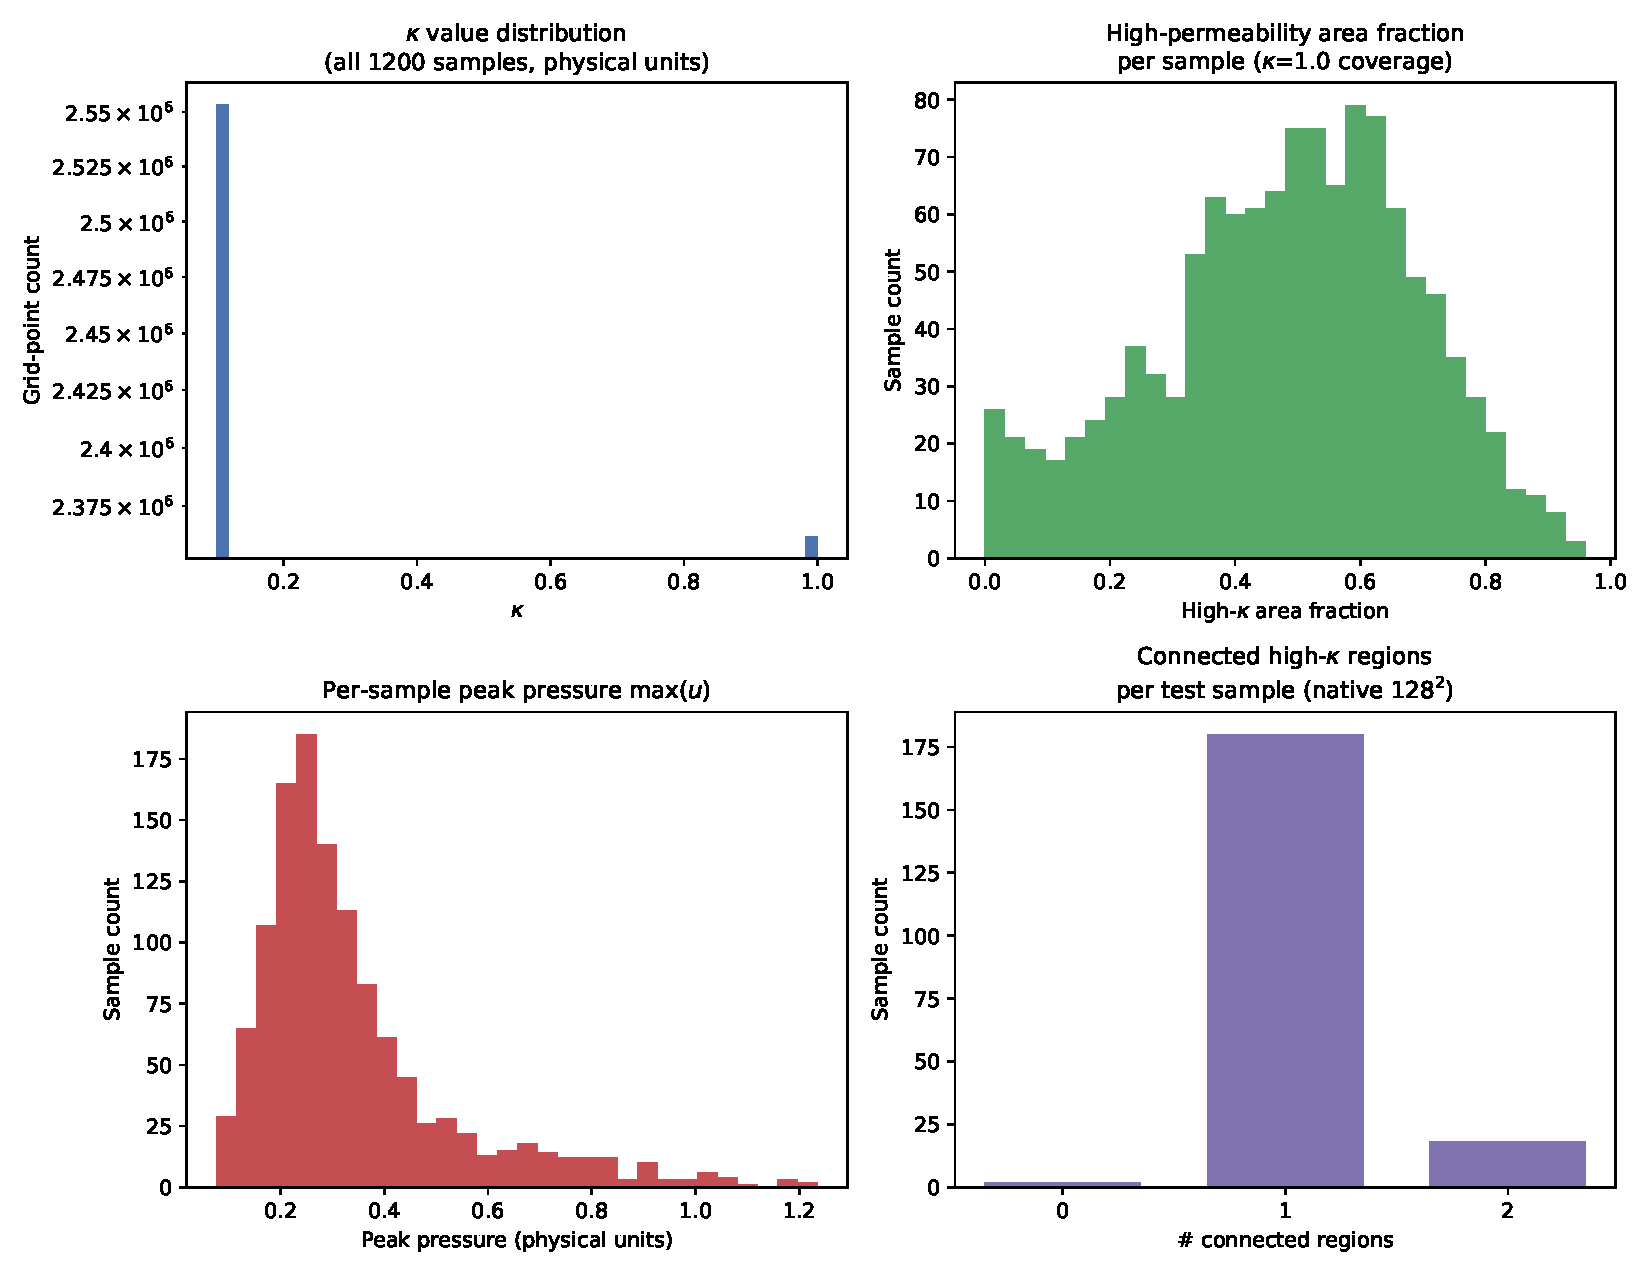
\includegraphics[width=0.55\textwidth]{figures/fig8_eda_dataset.pdf}
\caption{Dataset characterisation. $\kappa$ is exactly bimodal at $\{0.1,1.0\}$; the high-permeability area fraction varies widely (mean $0.48\pm0.21$); peak pressure has mean $0.34\pm0.19$ (physical units). At native $128\times128$, 180/200 test samples contain exactly one connected high-$\kappa$ region, 18/200 contain two, and 2/200 are exactly uniform ($\kappa\equiv0.1$, zero regions).}
\label{fig:eda}
\end{figure}

Three observations shape the modelling. (i) The permeability alphabet is binary, so sample-to-sample diversity comes from the \emph{shape and area} of the high-permeability region, not from its value. (ii) Samples are almost always a single blob (multi-region fields are rare), so the dataset is geometrically simple but the pressure amplitude varies strongly across samples (peak pressure ranges from about 0.1 to over 1.0). (iii) A few samples are exactly uniform in $\kappa$; these are rare edge cases that we track separately in the results (Section~\ref{sec:results}).

\subsection{Preprocessing Ablation (MLP)}
\label{sec:preabl}
To check that the preprocessing choices are sensible rather than assumed, we varied one choice at a time on the MLP baseline and retrained from scratch with three seeds each, on exactly the same split and target (so the test error is directly comparable). Table~\ref{tab:preabl} and Figure~\ref{fig:preabl} give the results.

\begin{table}[H]
\centering
\caption{MLP preprocessing ablation: test mean relative $L_2$ (200 samples), mean $\pm$ std over 3 seeds (\texttt{results/ablation\_preprocess.json}).}
\label{tab:preabl}
\begin{tabular}{lr}
\toprule
Preprocessing variant & Test mean rel.\ $L_2$ \\
\midrule
Reference: standardised inputs and targets, $+$ coordinates & $0.0842 \pm 0.0002$ \\
No coordinate channels ($\kappa$ only)                      & $0.0843 \pm 0.0011$ \\
No input normalisation (raw $\kappa$)                       & $0.0864 \pm 0.0018$ \\
No target normalisation (raw pressure)                      & $0.0917 \pm 0.0012$ \\
\bottomrule
\end{tabular}
\end{table}

\begin{figure}[H]
\centering
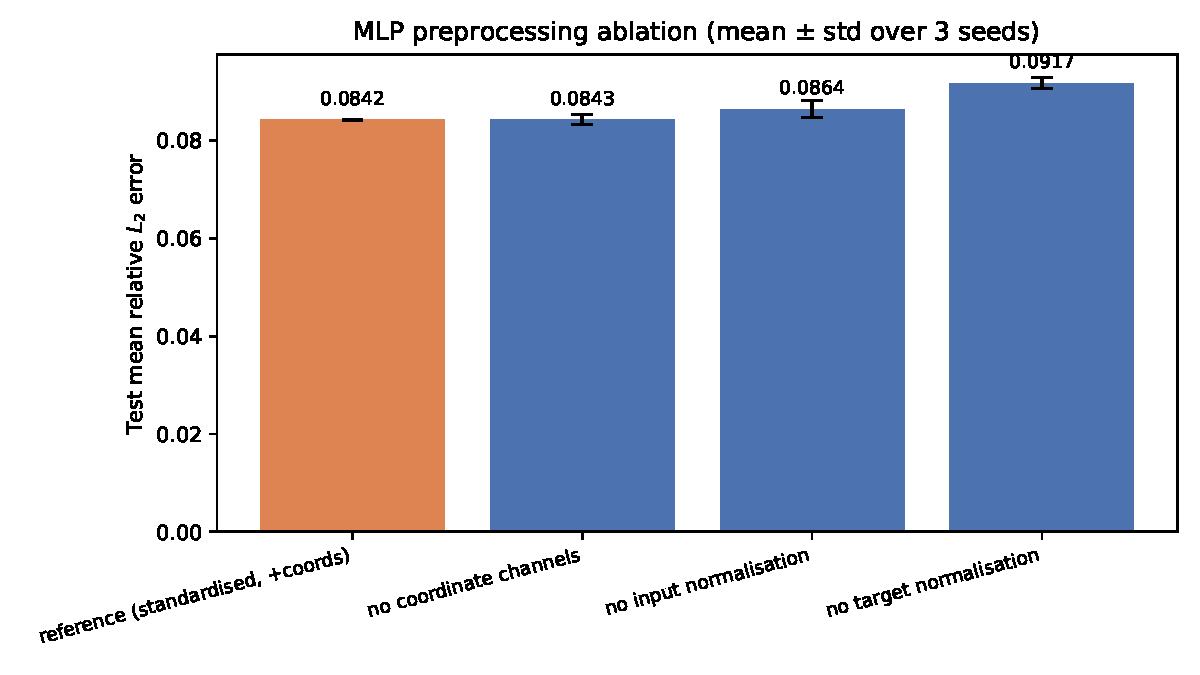
\includegraphics[width=0.46\textwidth]{figures/fig10_preprocess_ablation.pdf}
\caption{MLP preprocessing ablation (mean $\pm$ std over 3 seeds).}
\label{fig:preabl}
\end{figure}

Normalising the target is the choice that matters ($+9\%$ error without it, several seed-standard-deviations outside the reference). Input normalisation helps slightly. Coordinate channels make no measurable difference for the MLP (its flattened input already fixes each pixel's position); we keep them because they are the standard FNO input convention and give the two models identical inputs.

% ─────────────────────────────────────────────────────────────────────────────
\section{Model Architectures}

\subsection{MLP Baseline}
The MLP baseline flattens the $64\times64\times3$ input into a vector of 12,288 features and applies three hidden layers of width 2048 with GELU activations:
\[
  \text{MLP}: \mathbb{R}^{12288} \xrightarrow{2048} \xrightarrow{2048} \xrightarrow{2048} \mathbb{R}^{4096} \to \mathbb{R}^{64\times64},
\]
with a final linear projection. Total parameters: $\approx 42$\,M. The MLP is fixed to the training resolution ($64\times64$) and cannot generalise to other grid sizes.

\subsection{Fourier Neural Operator (FNO)}
The FNO \cite{li2021fno} processes the input as a $64\times64\times3$ field tensor through five stages:
\begin{enumerate}[nosep]
  \item \textbf{Lifting}: a pointwise linear layer maps 3 input channels to 64 hidden channels.
  \item \textbf{Four Spectral Convolution Blocks}: each block computes (i) a 2D FFT of the 64-channel field, (ii) retains only the lowest 12 Fourier modes in each direction ($12\times12$ complex-valued coefficients), (iii) multiplies by learned complex weights of shape $64\times64\times12\times12$, (iv) applies an inverse FFT, and (v) adds a pointwise local convolution bypass (equivalent to a $1\times1$ convolution).
  \item \textbf{Projection}: two linear layers ($64\to128\to1$) map hidden channels to the scalar output.
\end{enumerate}
Because the learned weights operate in frequency space (not on a fixed grid), the same trained network can in principle be evaluated at other grid resolutions, a property we plan to test in Stage 3. Total parameters: $\approx 4.7$\,M.

% ─────────────────────────────────────────────────────────────────────────────
\section{Training Protocol}

Both models are trained with:
\begin{itemize}[nosep]
  \item \textbf{Loss}: mean-squared error between the predicted and true standardised pressure fields.
  \item \textbf{Reported metric}: relative $L_2$ error $\|{\hat{u} - u}\|_2 / \|{u}\|_2$ per sample, computed after converting back to physical units (Section~\ref{sec:issues}).
  \item \textbf{Optimiser}: AdamW (decoupled weight decay $10^{-4}$), peak learning rate $10^{-3}$, with PyTorch's \texttt{CosineAnnealingLR} ($T_{\max}=100$) advanced once per mini-batch step. The learning rate therefore cycles between $10^{-3}$ and $0$ every 200 optimiser steps (about 3.5 epochs, $\sim$28 cycles per run), i.e.\ a warm-restart-like schedule rather than a single decay; it is identical for every model and ablation, so comparisons are like-for-like.
  \item \textbf{Batch size / epochs}: 16 / 100. No early stopping: every run completes its full epoch budget and the checkpoint with the lowest validation relative-$L_2$ error is retained (best epochs 92 for the FNO and 99 for the MLP).
\end{itemize}

% ─────────────────────────────────────────────────────────────────────────────
\section{MLP Baseline Ablation: Depth and Optimiser}
\label{sec:mlpabl}
The reported baseline (3 hidden layers of 2048, AdamW) was compared against shallower and differently-optimised variants, each retrained from scratch on the same data, split, loss and schedule (\texttt{src/ablation\_mlp.py}). Table~\ref{tab:mlpabl} and Figure~\ref{fig:mlpabl} report whatever the test set gives.

\begin{table}[H]
\centering
\caption{MLP baseline ablation, 200 test samples, single run per configuration (\texttt{results/ablation\_mlp.json}).}
\label{tab:mlpabl}
\begin{tabular}{lrrr}
\toprule
Configuration & Params & Mean rel.\ $L_2$ & Median \\
\midrule
1 hidden layer (2048), AdamW                 & 33.6\,M & 0.1008 & 0.0892 \\
2 hidden layers (2048$\times$2), AdamW        & 37.8\,M & 0.0796 & 0.0649 \\
3 hidden layers (2048$\times$3), AdamW (final) & 42.0\,M & 0.0857 & 0.0700 \\
3 hidden layers (2048$\times$3), SGD+momentum  & 42.0\,M & 0.1209 & 0.1091 \\
\bottomrule
\end{tabular}
\end{table}

\begin{figure}[H]
\centering
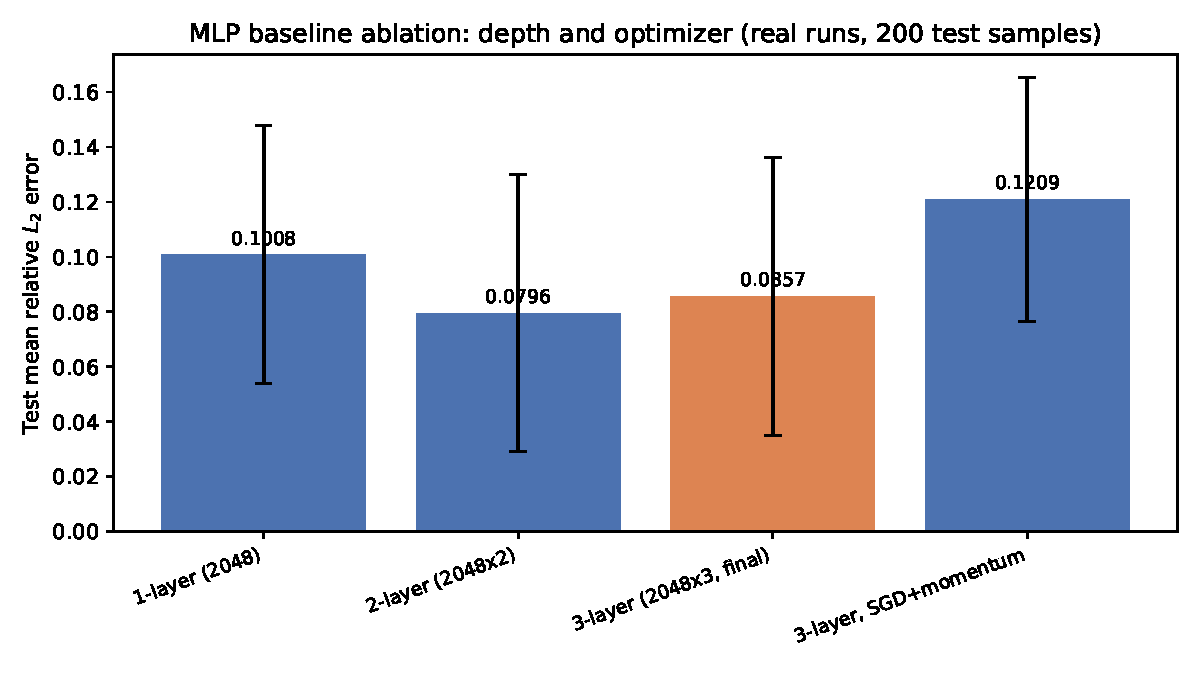
\includegraphics[width=0.46\textwidth]{figures/fig7_mlp_ablation.pdf}
\caption{MLP baseline ablation (error bars: one standard deviation across the 200 test samples).}
\label{fig:mlpabl}
\end{figure}

Two clear conclusions: a single hidden layer is too weak, and SGD with momentum is much worse than AdamW ($0.1209$ vs.\ $0.0857$), which justifies the optimiser choice. Depth beyond two layers brings no benefit at this dataset size: the 2-layer variant is marginally better than the 3-layer one, but a gap of $\sim0.006$ is of the same order as the run-to-run variation we measured ($\sim0.004$, Section~\ref{sec:issues}), so we treat 2 and 3 layers as equivalent. We keep the 3-layer network as the baseline because it was fixed before this study; it is therefore a fair, not a deliberately weak, comparison point for the FNO.

% ─────────────────────────────────────────────────────────────────────────────
\section{Preliminary Quantitative Results}
\label{sec:results}

All metrics are computed on the held-out 200-sample test set. Error is relative $L_2$: $\epsilon_{\rm rel} = \|{\hat{u} - u}\|_2 / \|{u}\|_2$ in physical units.

\begin{table}[H]
\centering
\caption{Test-set performance at training resolution ($64\times64$). Lower is better.}
\label{tab:results}
\begin{tabular}{lrrrrrr}
\toprule
Model & Params & Mean & Median & Std & Min & Max \\
\midrule
MLP baseline   & 42.0\,M & 0.0820 & 0.0695 & 0.0456 & 0.0325 & 0.3367 \\
FNO            &  4.7\,M & \textbf{0.0521} & \textbf{0.0398} & 0.0451 & \textbf{0.0155} & 0.3467 \\
\bottomrule
\end{tabular}
\end{table}

Key observations:
\begin{enumerate}[nosep]
  \item The FNO achieves $36\%$ lower mean error than the MLP while using $9\times$ fewer parameters, demonstrating the advantage of spectral inductive biases for smooth PDE solutions.
  \item Both models have right-skewed error distributions: most samples have errors well below 0.1, while a small fraction ($\lesssim5\%$) pushes the error toward 0.3 (Figure~\ref{fig:hist}). The maximum error is similar for the two models, so the FNO's advantage is in the bulk of the distribution rather than the tail.
  \item The single worst FNO test sample is not a complex field but the opposite: a perfectly uniform permeability field (Figure~\ref{fig:samples}, bottom row).
\end{enumerate}

\begin{figure}[H]
\centering

\includegraphics[width=0.5\textwidth]{figures/fig1_error_histogram.pdf}
\caption{Error distribution across 200 test samples. Dashed vertical lines indicate per-model means. FNO errors are concentrated at lower values; the MLP's distribution is shifted right.}
\label{fig:hist}
\end{figure}

\begin{figure}[H]
\centering
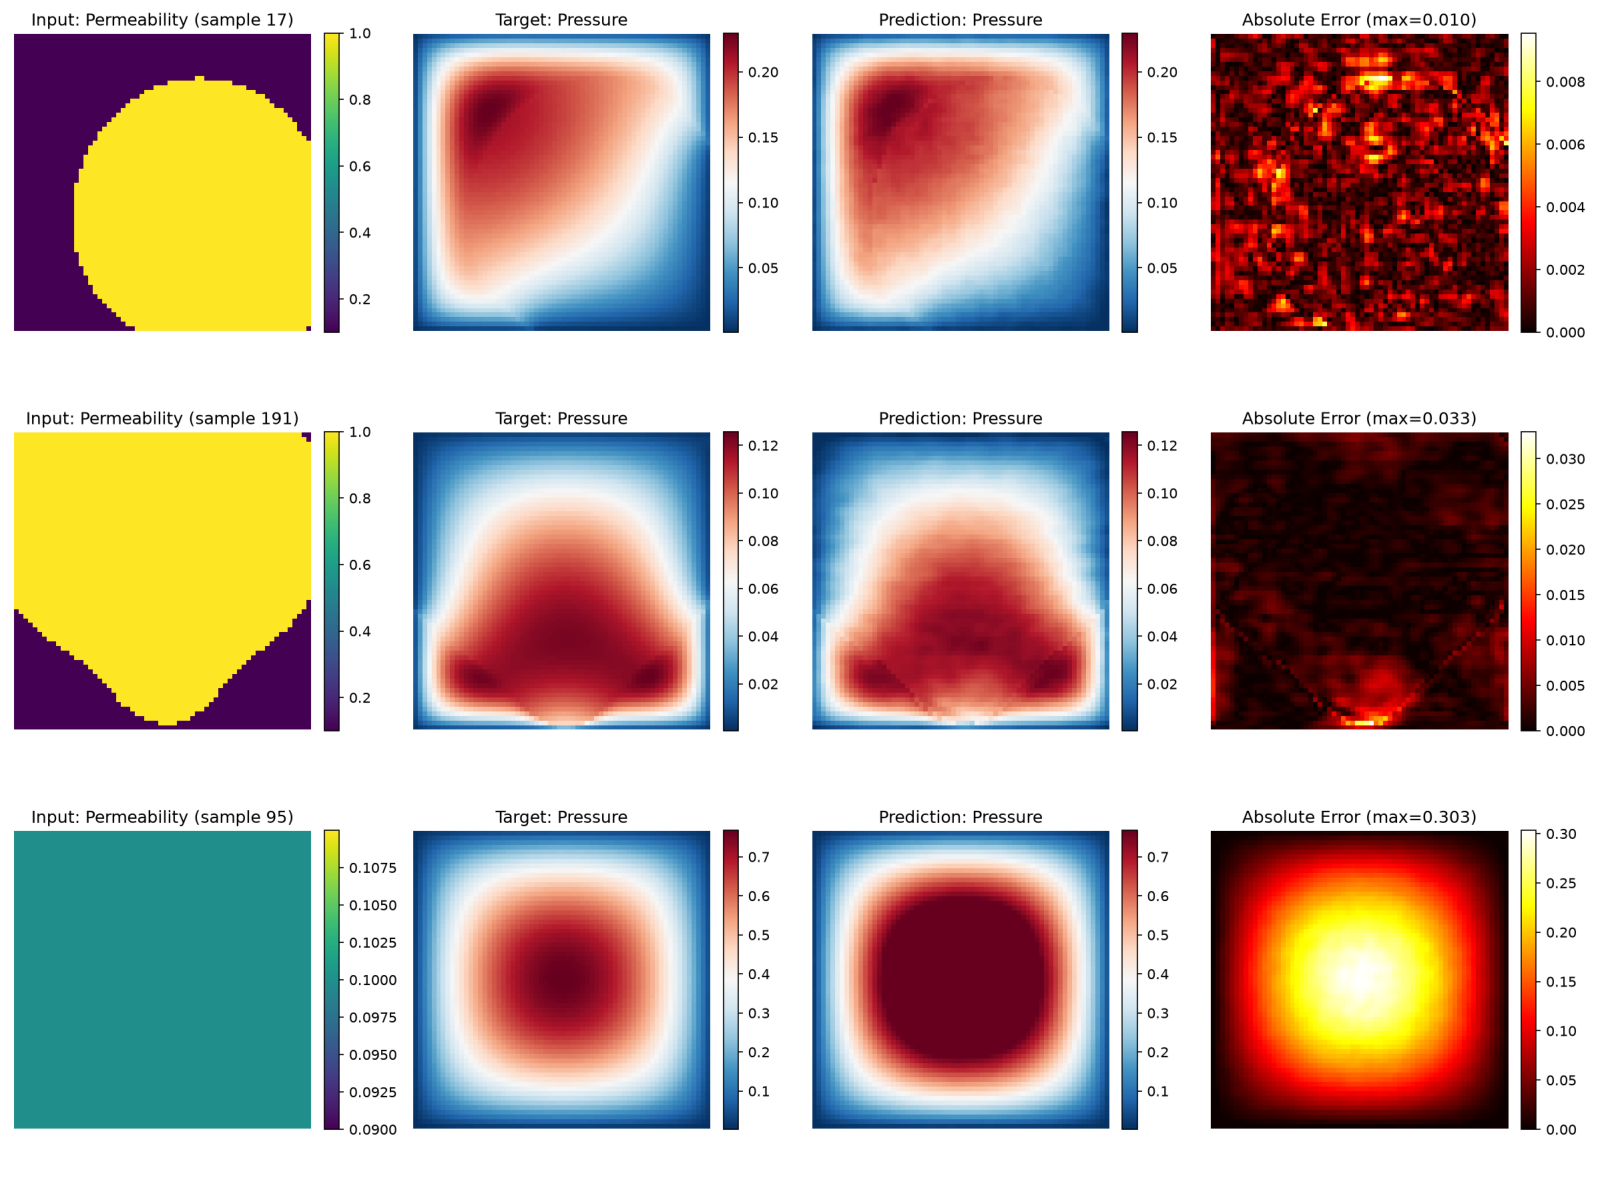
\includegraphics[width=0.78\textwidth]{figures/fig_sample_predictions.png}
\caption{FNO predictions for the best (sample 17, error 0.016), a median-error (sample 191, error 0.040) and the worst (sample 95, error 0.347) test sample. Columns: input $\kappa$, target pressure, predicted pressure, absolute error. The worst case has exactly uniform $\kappa\equiv0.1$: the true pressure is a smooth bump, but the FNO over-predicts its amplitude (the prediction saturates the colour scale of the target) --- a failure mode specific to this degenerate input.}
\label{fig:samples}
\end{figure}

% ─────────────────────────────────────────────────────────────────────────────
\section{Code Quality and Reproducibility}

The codebase is organised into four directories:
\begin{itemize}[nosep]
  \item \texttt{src/} - \texttt{download\_data.py} and \texttt{preprocess.py} (checksum-verified download, split and normalisation), \texttt{models.py} (\texttt{MLPBaseline}, \texttt{SpectralConv2d}, \texttt{FNO2d}), \texttt{train.py} (training loop; keeps the best-validation checkpoint), \texttt{evaluate.py} (test metrics and sample plots), \texttt{eda.py}, \texttt{ablation\_mlp.py}, \texttt{ablation\_preprocess.py}.
  \item \texttt{configs/} - \texttt{fno.yaml}, \texttt{mlp.yaml}.
  \item \texttt{results/} - one \texttt{run\_00x/} per model with its \texttt{eval\_metrics.json}, plus the ablation and EDA outputs and \texttt{figures/}.
  \item \texttt{tests/} - the \texttt{pytest} suite.
\end{itemize}
A \texttt{pytest} suite covers model shapes, the relative-$L_2$ metric, and data loading; all results are committed. Training and evaluation reproduce with:
\begin{verbatim}
python3 src/download_data.py
python3 src/preprocess.py
python3 src/train.py    --config configs/fno.yaml
python3 src/evaluate.py --config configs/fno.yaml \
    --checkpoint results/run_001/best_model.pt
\end{verbatim}
\textbf{Platform.} Everything is run as plain Python scripts (no Colab/Kaggle notebooks): code development and checks on a local macOS (Apple Silicon, MPS) machine, and training on a remote Linux workstation with an NVIDIA RTX PRO 6000 GPU (CUDA) accessed over SSH. The random seed is fixed to 42 for the data split, and, in the current code, for model initialisation and batch order as well.

% ─────────────────────────────────────────────────────────────────────────────
\section{Issues Encountered}
\label{sec:issues}

\begin{enumerate}[nosep]
  \item \textbf{Metric convention.} Relative $L_2$ must be computed in physical units. Computed on standardised fields, the subtracted mean changes $\|u\|_2$ (but not $\|\hat u-u\|_2$), so the number is not comparable with the literature. All reported errors are computed after de-normalising, and the metric is unit-tested.
  \item \textbf{Uniform-permeability samples.} Exactly uniform $\kappa$ fields (2 of the 200 test samples) are a degenerate input on which the FNO over-predicts the pressure amplitude; one of them is the worst test sample (error 0.347, Figure~\ref{fig:samples}). We report this failure openly rather than excluding those samples.
  \item \textbf{Compute constraints.} The raw PDEBench file is 1.3\,GB; loading it and training the 42\,M-parameter MLP and the FNO for 100 epochs (plus the ablations) was moved to the lab GPU workstation, while code development and unit tests stayed on the local machine.
  \item \textbf{Run-to-run variance.} The first training runs (the reported \texttt{run\_001}/\texttt{run\_002}) did not fix the model-initialisation seed. Re-training the identical MLP configuration gives errors differing by $\sim0.004$ (e.g.\ $0.0820$ reported vs.\ $0.0857$ in Section~\ref{sec:mlpabl}), which we treat as the noise floor: only gaps larger than this are interpreted. The training code now seeds Python, NumPy and PyTorch, and the preprocessing ablation above uses 3 fixed seeds per variant.
\end{enumerate}

% ─────────────────────────────────────────────────────────────────────────────
\section{Future Work (Stage 3)}
\label{sec:future}

The following are planned for the final stage:
\begin{enumerate}[nosep]
  \item \textbf{FNO scaling study.} Train larger FNO configurations (more width, Fourier modes and blocks) and vary modes and width systematically to map the accuracy--parameter trade-off against the MLP baseline.
  \item \textbf{Resolution generalisation.} Evaluate the trained FNO zero-shot at the native $128\times128$ resolution using the native-resolution test fields already set aside during preprocessing, and compare it with an FNO trained directly at $128\times128$.
  \item \textbf{Computational cost.} Benchmark inference time of both models against the finite-difference reference solver, and profile the cost of the individual FNO operations (FFT, spectral multiplication, local convolution).
  \item \textbf{Physical interpretation.} Quantify how the per-sample error relates to the geometry of the permeability field (number of regions, interface length, area fraction), including the uniform-$\kappa$ failure cases identified above.
  \item \textbf{Learning-rate schedule.} Compare the current per-step cosine cycling with standard per-epoch cosine annealing, to check how much of the remaining error is optimisation rather than model capacity.
  \item \textbf{Final deliverables.} Final report, contribution statement and AI-tool-use declaration, final presentation, and viva.
\end{enumerate}

% ─────────────────────────────────────────────────────────────────────────────
\begin{thebibliography}{9}
\bibitem{li2021fno}
  Z.\ Li et al., ``Fourier Neural Operator for Parametric Partial Differential Equations,'' \textit{ICLR}, 2021.

\bibitem{takamoto2022pdebench}
  M.\ Takamoto et al., ``PDEBench: An Extensive Benchmark for Scientific Machine Learning,'' \textit{NeurIPS}, 2022. DOI: 10.18419/darus-2986.
\end{thebibliography}

\end{document}
